\begin{figure*}[!htbp]
    \centering
    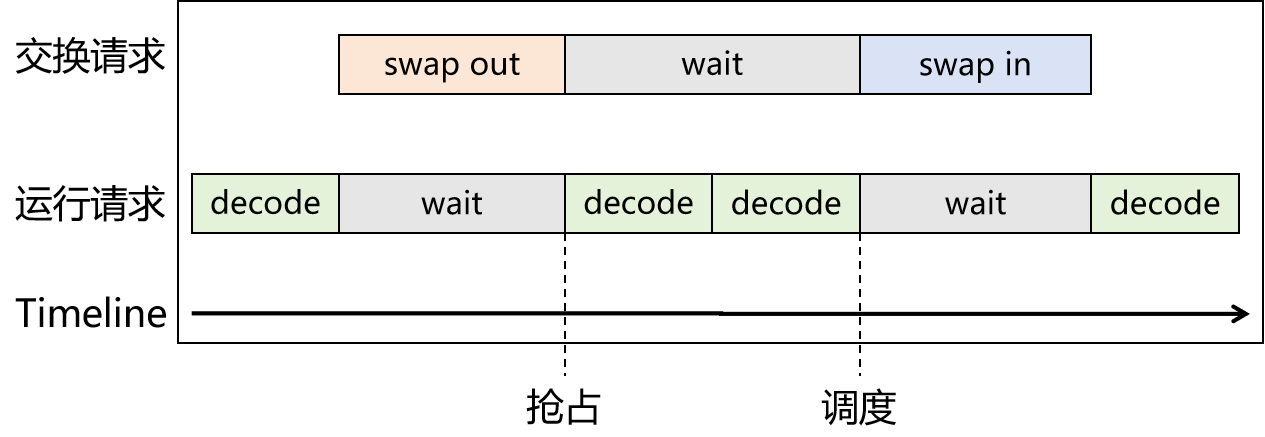
\includegraphics[width=1\linewidth]{张量交换示意图.png}
    \caption{张量交换示意图} 
    \label{Fig:张量交换示意图}
  \end{figure*}

\section{相关工作}

\subsubsection{张量交换技术}

随着批处理大小的增加或模型参数量的扩展,运行时需要保存的张量会超出GPU内存限制。张量交换技术在GPU空间不足时开启,将一部分需要保存,而暂时用不到的张量换出至CPU中,在计算需要时重新换入GPU中。图\ref{Fig:张量交换示意图}展示了张量交换的基本流程。

HuggingFace Accelerate~\cite{Huggingface-Accelerate}实现了张量交换技术,但换出与换入的张量仅限于LLM的参数张量。LightLLM~\cite{LightLLM}能够针对KV Cache进行张量交换,但换出的比例设计为定值,无法根据运行时信息调整。

FlexGen~\cite{Swapping}首次提出了“自适应内存优化”的概念,通过线性规划建模在交换方案的可行域内进行搜索,在给定的时间限制内找到一个较优解。然而,FlexGen假设运行队列中的所有用户请求拥有相同的输出长度。在实际情况下,输出长度具有很大的差异性,使得相关理论无法推广。

本文针对KV Cache实现张量交换技术,并进行细粒度内存占用建模分析。根据GPU内存使用水平,进行实时换出换入调整。

\subsubsection{张量重算技术}

Mimose~\cite{Recomputation, Recomp_2, Recomp_3}等工作提出了张量重算技术。在抢占式用户请求调度系统中,当某个请求获得执行权时,会检查之前的计算结果是否保存在GPU中,如果不在,则需要重新获取这部分计算结果。图\ref{Fig:张量重算示意图}展示了张量重算的基本流程。

\begin{figure}[!htbp]
  \centering
  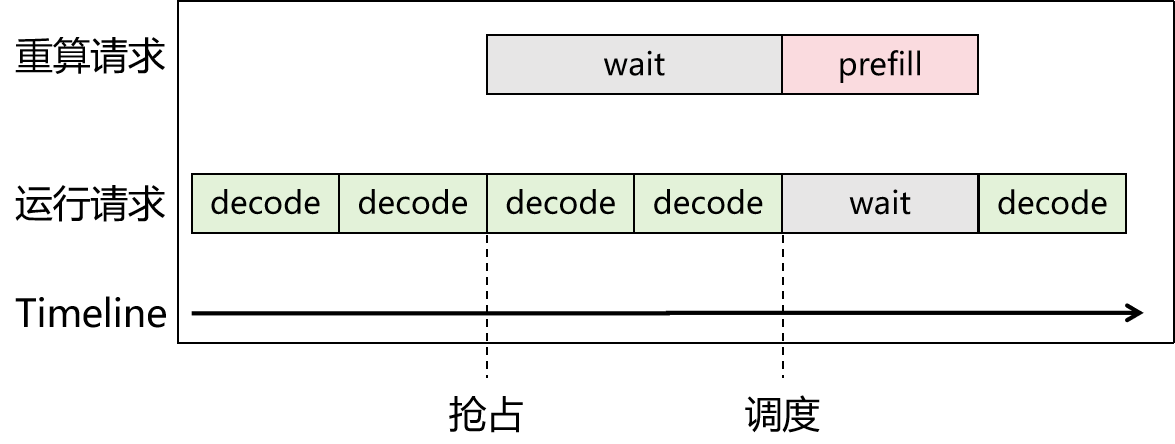
\includegraphics[width=1\linewidth]{张量重算示意图.png}
  \caption{张量重算示意图} 
  \label{Fig:张量重算示意图}
\end{figure}

张量重算开销的计算相比于张量交换略微复杂。Capuchin~\cite{Capuchin}将张量重算开销计算过程分解到算子粒度。对于每个算子,通过记录其输入张量与输出张量的生成时间,来获取该算子的重算开销。AdaPipe~\cite{AdaPipe}将连续出现的多个算子组合成计算单元,通过模拟运行来记录各个计算单元的重算开销。

本文针对KV Cache实现张量重算技术。这些key-value张量在初次生成时经历了多次前向传播,而在重算过程中仅需调用自注意力机制即可得到,因此张量重算的开销远远小于token序列初次生成时的开销,不会导致计算量的爆炸式增长。

\subsubsection{LLM推理优化技术}

除了张量交换和张量重算等针对张量层面的优化策略以外,传统LLM推理服务框架还采用了很多其它的推理优化技术。

ORCA~\cite{ORCA}将批处理调度的粒度从单个用户请求转化为单次推理迭代,化解了用户请求相互等待的性能瓶颈。vLLM~\cite{vLLM}基于OS页式内存管理思想,在ORCA的基础上引入Paged Attention机制。vLLM相比于OCRA,大幅度提升显存利用率,增加批处理大小上限,进而提升推理任务的整体吞吐率。

SpecInfer~\cite{SpecInfer}引入了投机推理技术(Speculative Sampling),根据小型LLM模型的输出来预测大型LLM模型的输出,在大幅度提升推理吞吐率的同时保障了输出质量。DistillSpec~\cite{DistillSpec}在SpecInfer的基础上实现了知识蒸馏技术(Knowledge Distillation,KD),使得输出预测的准确率显著提升。

本文提出的LLM推理优化策略能够与调度粒度转化、投机推理等研究工作相兼容。本文设计了规范且友好的用户接口,开发者能够根据任务需求来定义各种参数,极大地方便了有关推理优化的深入研究。
